\documentclass[12pt]{article}
\usepackage[margin=1in]{geometry}
\usepackage{amsmath,amssymb,amsthm,booktabs,graphicx,natbib,microtype}
\newtheorem{theorem}{Theorem}
\newtheorem{corollary}[theorem]{Corollary}
\newtheorem{proposition}[theorem]{Proposition}
\newtheorem{remark}[theorem]{Remark}
\title{Outward Finite Directional Composition\\\large Two Loewner Residuals, a Precision Barrier, and 28 Validated Packet Chains}
\author{Prime Dynamics Theory Program}
\date{July 2026}

\begin{document}
\maketitle

\begin{abstract}
RH-137 produced a composable finite-horizon upper envelope $D_t\preceq
y_tG_t$ on 28 of 30 packet chains, but its audit used one high-precision
assembly path.  We give an outward validation layer that can be checked from
independently rounded matrices and spectral-norm radii.  For a raw recurrence
\[
 D'\preceq rO^*DO+F
\]
and a source certificate $D\preceq yG$, two guarded residuals suffice:
\[
 rO^*\widehat DO+\widehat F-\widehat D',
 \qquad
 y'\widehat G'-ryO^*\widehat GO-\widehat F.
\]
We derive the exact outward losses for both residuals and prove scalar
sharpness.  Their certification implies $D'\preceq y'G'$ without fusing
unguarded assemblies.

The normalized directional base also admits a direct outward lower.  If
$\|G-\widehat G\|\leq r_G$, then
\[
 \frac{\sqrt{\det G}}{L^4C}
 =\sqrt{\frac{\lambda_{\min}(G)}{\lambda_{\max}(G)}}
 \geq
 \sqrt{\frac{(\lambda_{\min}(\widehat G)-r_G)_+}
 {\lambda_{\max}(\widehat G)+r_G}}.
\]
Combining this with the validated tail envelope gives an explicit
directional support lower.

On the frozen 80-decimal reference assembly, we round every matrix
independently to 40 decimal digits and archive its norm radius.  All 330 raw
recurrence and normalized bridge residuals certify outwardly, with zero tail
or support dominance failures.  The directional lower is positive on
328/330 transitions and 28/30 chains; 21 terminal lowers exceed $10^{-8}$.
The largest forcing padding is $2.28\times10^{-45}$ and the largest additive
tail-bound inflation is $2.58\times10^{-23}$.  A sharp precision barrier is
also visible: fp64 norm balls retain a positive base on only 320 snapshots,
16-digit decimal balls on 318, 18-digit balls on 324, and 20-digit balls on
all 330.  This closes the finite reference-assembly validation layer, but it
does not provide interval enclosures for the underlying source model or an
all-level positive base law.
\end{abstract}

\section{The two-residual validation problem}
Let $G,G'\succ0$ be source and target recent Gramians and let $D,D'\succeq0$
be their weighted memory tails.  A moving-frame step supplies an orthogonal
map $O$, a raw factor $r\geq0$, and positive forcing $F$ such that
\begin{equation}\label{eq:raw}
 D'\preceq rO^*DO+F.
\end{equation}
Suppose a previous step has already certified
\begin{equation}\label{eq:source}
 D\preceq yG.
\end{equation}
To propagate this certificate it is enough to prove
\begin{equation}\label{eq:bridge}
 ryO^*GO+F\preceq y'G'.
\end{equation}
Equations \eqref{eq:raw}--\eqref{eq:bridge} then give
$D'\preceq y'G'$ by transitivity.

In computation, however, the five matrices may be assembled and rounded
independently.  Write hats for archived approximations and assume spectral
norm radii
\[
 \|G-\widehat G\|\leq r_G,
 \quad \|D-\widehat D\|\leq r_D,
 \quad \|G'-\widehat G'\|\leq r_{G'},
 \quad \|D'-\widehat D'\|\leq r_{D'},
 \quad \|F-\widehat F\|\leq r_F.
\]
The residuals must be reduced by the worst error allowed by these balls.

\section{Outward recurrence and bridge guards}
\begin{theorem}[Two-residual outward composition]\label{thm:two}
Define the numerical minimum-eigenvalue slacks
\begin{align*}
 \widehat\mu_R
 &=\lambda_{\min}(rO^*\widehat DO+\widehat F-\widehat D'),\\
 \widehat\mu_B
 &=\lambda_{\min}(y'\widehat G'-ryO^*\widehat GO-\widehat F).
\end{align*}
If
\begin{align}
 \widehat\mu_R&\geq r\|O\|^2r_D+r_F+r_{D'},\label{eq:rawguard}\\
 \widehat\mu_B&\geq y'r_{G'}+ry\|O\|^2r_G+r_F,\label{eq:bridgeguard}
\end{align}
then both \eqref{eq:raw} and \eqref{eq:bridge} hold.  Consequently,
\eqref{eq:source} implies $D'\preceq y'G'$.  The two guard constants are
individually sharp from norm radii alone.
\end{theorem}

\begin{proof}
The exact raw residual differs from the numerical one by
\[
 rO^*(D-\widehat D)O+(F-\widehat F)-(D'-\widehat D').
\]
Its norm is at most the right side of \eqref{eq:rawguard}.  Weyl's
minimum-eigenvalue perturbation inequality therefore proves positivity of
the exact raw residual.  The bridge residual differs by
\[
 y'(G'-\widehat G')-ryO^*(G-\widehat G)O-(F-\widehat F),
\]
whose norm is bounded by the right side of \eqref{eq:bridgeguard}.  This
proves the bridge.  In dimension one, choose every enclosure error with the
sign that decreases its residual; equality then holds in either guard, so
no smaller universal constants follow from the same radii
\citep{HornJohnson1991,Moore1966}.
\end{proof}

The theorem extends the RH-127 transport guard to an arbitrary positive
forcing matrix and adds the normalized bridge needed by RH-137.  It also
separates two logically distinct failures: the dynamical recurrence may be
invalid, or it may be valid but too large relative to the target Gram.

\begin{corollary}[Validated finite chain]\label{cor:chain}
If $D_0\preceq y_0G_0$ and both residual guards certify at every step, then
$D_t\preceq y_tG_t$ for the entire finite chain.
\end{corollary}

This is a direct induction.  No constant coefficient, asymptotic
contractivity, or common matrix assembly is required.

\section{Outward normalized base and support lower}
Let $K$ be the reduced recent action and let
$s_1\geq s_2\geq s_3\geq s_4>0$ be its singular values, so
$G=K^*K$.  Put
\[
 V=\sqrt{\det G}=s_1s_2s_3s_4,
 \qquad L=s_1,
 \qquad C=\frac{s_2s_3}{s_1^2}.
\]
The normalized frame/capacity factor from RH-125 simplifies exactly:
\begin{equation}\label{eq:baseidentity}
 \frac{V}{L^4C}=\frac{s_4}{s_1}
 =\sqrt{\frac{\lambda_{\min}(G)}{\lambda_{\max}(G)}}.
\end{equation}
Thus no separate volume and capacity enclosure is needed at a fixed
snapshot.

\begin{theorem}[Outward directional snapshot lower]\label{thm:support}
Assume $\|G-\widehat G\|\leq r_G$ and define
\[
 a_-(\widehat G,r_G)=
 \sqrt{\frac{(\lambda_{\min}(\widehat G)-r_G)_+}
 {\lambda_{\max}(\widehat G)+r_G}}.
\]
If $D\preceq yG$, then the directional candidate satisfies
\[
 B(G,D)\geq (1-\sqrt y)_+^4a_-(\widehat G,r_G).
\]
Both the eigenvalue endpoints and the fourth-power tail factor are sharp.
\end{theorem}

\begin{proof}
Weyl perturbation gives
$\lambda_{\min}(G)\geq\lambda_{\min}(\widehat G)-r_G$ and
$\lambda_{\max}(G)\leq\lambda_{\max}(\widehat G)+r_G$.  Insert these into
\eqref{eq:baseidentity}.  The Loewner inequality $D\preceq yG$ gives
$\gamma^2\leq y$ for the generalized top Rayleigh value, and the map
$(1-\gamma)_+^4$ is decreasing.  Diagonal endpoint perturbations and scalar
relative tails attain equality \citep{Bhatia1997}.
\end{proof}

\section{A sharp precision-information barrier}
The base lower is positive exactly when
$\lambda_{\min}(\widehat G)>r_G$.  Failure of this test is not merely a
weakness of Theorem~\ref{thm:support}.

\begin{proposition}[Norm-ball positivity barrier]\label{prop:precision}
If $\widehat G\succeq0$ and
$\lambda_{\min}(\widehat G)\leq r_G$, then the spectral-norm ball
$\{G:\|G-\widehat G\|\leq r_G\}$ contains a singular positive semidefinite
matrix.  Therefore no strictly positive lower for
$\sqrt{\lambda_{\min}(G)/\lambda_{\max}(G)}$ can be inferred from that
enclosure alone.
\end{proposition}

\begin{proof}
Let $v$ be a unit minimum eigenvector and set
$G_0=\widehat G-\lambda_{\min}(\widehat G)vv^*$.  Then $G_0\succeq0$ is
singular and lies within the stated radius.
\end{proof}

Hence extra arithmetic precision, a structured error model, or an
independent lower-gap theorem is genuinely necessary when the weakest Gram
direction falls inside the norm radius.

\section{Independently rounded finite audit}
We rebuild the 30 rank-four, depth-eight packet chains at 80 decimal digits.
Every source Gram, source tail, target Gram, target tail, and forcing matrix
is then rounded independently to 40 significant decimal digits.  Its
spectral-norm difference from the frozen reference matrix is archived as an
outward radius.  Small positive scalar padding is added to the forcing only
when needed to make \eqref{eq:rawguard} outward; $y'$ is then increased only
as needed for \eqref{eq:bridgeguard}.  This procedure validates the rounded
archive relative to the frozen reference assembly.  It is not an interval
construction of the upstream source model \citep{Higham2002}.

All 330 raw residuals and all 330 normalized bridges certify.  There are
zero failures of $D'\preceq y'G'$ and zero cases where the support lower
exceeds the directly evaluated reference candidate.  The maximum forcing
padding is $2.2742\times10^{-45}$; the largest additive increase in $y'$ is
$2.5758\times10^{-23}$.  Thus outward closure costs essentially nothing at
40 digits on this archive.

\begin{table}[t]
\centering
\begin{tabular}{rrrrrr}
\toprule
$\sigma$ & transitions & positive & $\geq10^{-8}$ & $\geq10^{-6}$ & $\geq10^{-4}$ \\
\midrule
0.16 & 18  & 18  & 6   & 0   & 0 \\
0.08 & 30  & 28  & 28  & 25  & 6 \\
0.04 & 60  & 60  & 59  & 55  & 40 \\
0.02 & 96  & 96  & 96  & 96  & 96 \\
0.01 & 126 & 126 & 126 & 126 & 126 \\
\midrule
total & 330 & 328 & 315 & 302 & 268 \\
\bottomrule
\end{tabular}
\caption{Outward-composed directional lower by scale.}
\label{tab:counts}
\end{table}

The 328 positive lowers range from $1.0366\times10^{-10}$ to $0.32144$,
with median $0.011966$.  Twenty-eight complete chains remain positive.  At
their terminal snapshots, 21 exceed $10^{-8}$, 16 exceed $10^{-6}$, and 12
exceed $10^{-4}$.  The two zero chains are exactly the RH-137 coarse
superunit-birth failures.

\begin{figure}[t]
\centering
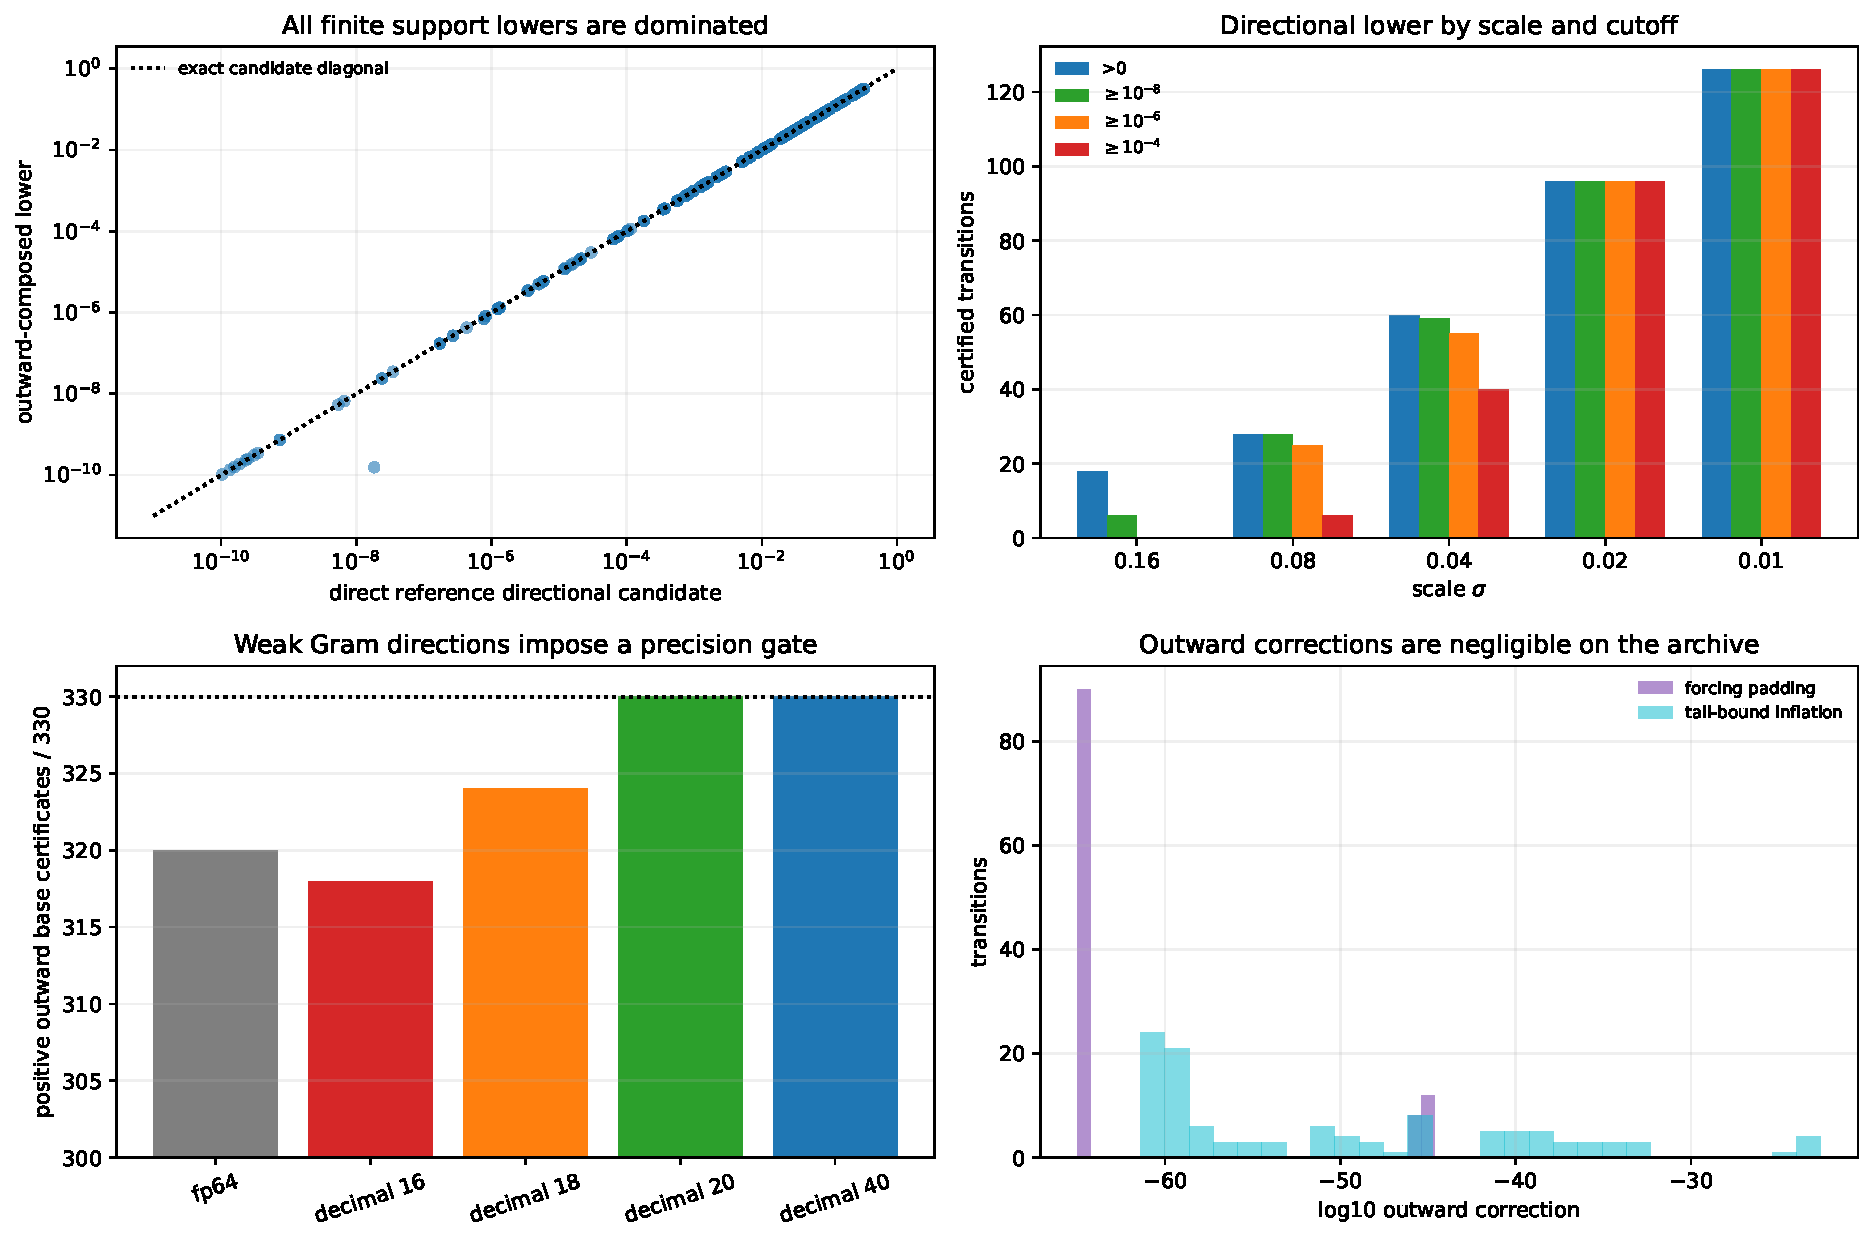
\includegraphics[width=\textwidth]{figures/outward_finite_directional_composition.pdf}
\caption{Support dominance, threshold counts, the arithmetic precision gate,
and the tiny outward corrections required by the rounded archive.}
\label{fig:audit}
\end{figure}

The precision sweep confirms Proposition~\ref{prop:precision}.  Direct fp64
rounding retains a positive norm-ball base on 320 of 330 snapshots.  Decimal
rounding to 16 significant digits retains 318, to 18 digits retains 324, and
to 20 digits retains all 330.  The lost fp64 cases are all coarse
$\sigma=0.16$ snapshots with exact normalized bases between
$1.04\times10^{-10}$ and $7.37\times10^{-10}$.  Forty digits are retained in
the archive to leave a large validation margin.

\section{Route consequence and boundary}
RH-138 completes a finite proof object that RH-125 and RH-127 only described
conditionally.  A verifier can reconstruct each step from rounded matrices,
radii, two residual slacks, and the target base endpoint.  The result keeps
the tail recurrence, normalization, and capacity on one assembly path and
does not use the earlier artificial positive Gram floor.

What remains is physical and asymptotic.  The 80-digit reference matrices
still originate from a floating packet/model assembly rather than an exact
or interval enclosure of that source.  The positive finite bases do not
prove a uniform positive liminf.  The finite-horizon policy does not yet
cover arbitrary future levels, and two coarse birth events remain superunit.

We have not proved source-model interval radii, all-level outward residuals,
a uniform positive base law, uniform Stage A, a Hilbert--Polya operator,
zeta-zero identification, or the Riemann Hypothesis.

\bibliographystyle{plainnat}
\bibliography{references}
\end{document}
